\documentclass{article}
\usepackage[x11names, svgnames, rgb]{xcolor}
\usepackage[utf8]{inputenc}
\usepackage{tikz}
\usetikzlibrary{snakes,arrows,shapes}
\usepackage{amsmath}
%
%

%

%

\begin{document}
\pagestyle{empty}
%
%
%

\enlargethispage{100cm}
% Start of code
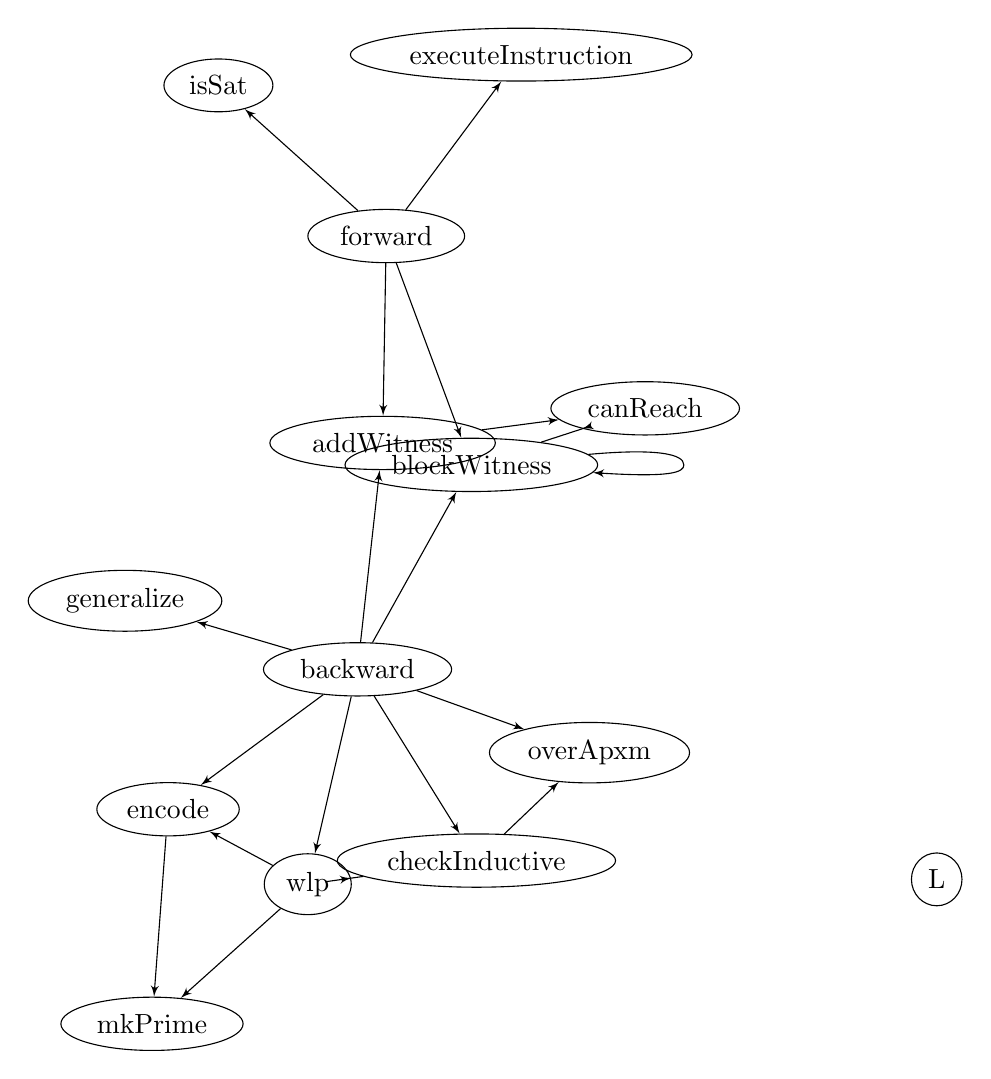
\begin{tikzpicture}[>=latex',line join=bevel,]
%%
\node (eL) at (339.0bp,70.0bp) [draw,ellipse] {\text{L}};
  \node (encode) at (62.28bp,95.24bp) [draw,ellipse] {encode};
  \node (mkPrime) at (56.501bp,18.0bp) [draw,ellipse] {mkPrime};
  \node (wlp) at (112.58bp,68.255bp) [draw,ellipse] {wlp};
  \node (forward) at (140.83bp,301.59bp) [draw,ellipse] {forward};
  \node (executeInstruction) at (189.42bp,366.9bp) [draw,ellipse] {executeInstruction};
  \node (isSat) at (80.416bp,355.83bp) [draw,ellipse] {isSat};
  \node (addWitness) at (139.52bp,227.11bp) [draw,ellipse] {addWitness};
  \node (blockWitness) at (171.47bp,219.21bp) [draw,ellipse] {blockWitness};
  \node (canReach) at (234.05bp,239.57bp) [draw,ellipse] {canReach};
  \node (backward) at (130.5bp,145.61bp) [draw,ellipse] {backward};
  \node (overApxm) at (214.0bp,115.61bp) [draw,ellipse] {overApxm};
  \node (checkInductive) at (173.3bp,76.762bp) [draw,ellipse] {checkInductive};
  \node (generalize) at (46.796bp,170.29bp) [draw,ellipse] {generalize};
  \draw [->] (encode) ..controls (60.227bp,67.797bp) and (59.384bp,56.537bp)  .. (mkPrime);
  \draw [->] (wlp) ..controls (91.447bp,79.593bp) and (91.353bp,79.644bp)  .. (encode);
  \draw [->] (wlp) ..controls (92.051bp,49.857bp) and (87.284bp,45.585bp)  .. (mkPrime);
  \draw [->] (forward) ..controls (158.61bp,325.49bp) and (164.48bp,333.37bp)  .. (executeInstruction);
  \draw [->] (forward) ..controls (117.26bp,322.76bp) and (110.75bp,328.6bp)  .. (isSat);
  \draw [->] (forward) ..controls (140.36bp,275.12bp) and (140.18bp,264.85bp)  .. (addWitness);
  \draw [->] (forward) ..controls (151.47bp,273.0bp) and (156.62bp,259.13bp)  .. (blockWitness);
  \draw [->] (addWitness) ..controls (188.3bp,233.54bp) and (188.44bp,233.56bp)  .. (canReach);
  \draw [->] (blockWitness) ..controls (238.72bp,225.24bp) and (247.97bp,223.04bp)  .. (247.97bp,219.21bp) .. controls (247.97bp,216.52bp) and (243.4bp,214.63bp)  .. (blockWitness);
  \draw [->] (blockWitness) ..controls (211.86bp,232.35bp) and (211.9bp,232.37bp)  .. (canReach);
  \draw [->] (backward) ..controls (103.12bp,125.39bp) and (96.76bp,120.7bp)  .. (encode);
  \draw [->] (backward) ..controls (124.17bp,118.29bp) and (121.47bp,106.61bp)  .. (wlp);
  \draw [->] (backward) ..controls (133.64bp,174.03bp) and (135.1bp,187.23bp)  .. (addWitness);
  \draw [->] (backward) ..controls (145.26bp,172.13bp) and (151.19bp,182.79bp)  .. (blockWitness);
  \draw [->] (backward) ..controls (165.66bp,132.97bp) and (167.37bp,132.36bp)  .. (overApxm);
  \draw [->] (backward) ..controls (146.18bp,120.39bp) and (151.7bp,111.51bp)  .. (checkInductive);
  \draw [->] (backward) ..controls (93.926bp,156.39bp) and (93.824bp,156.42bp)  .. (generalize);
  \draw [->] (checkInductive) ..controls (115.45bp,68.657bp) and (115.4bp,68.649bp)  .. (wlp);
  \draw [->] (checkInductive) ..controls (191.84bp,94.459bp) and (191.94bp,94.55bp)  .. (overApxm);
%
\end{tikzpicture}
% End of code

%
\end{document}
%



